\documentclass[14pt,a4paper]{extreport}

\usepackage{style/style}
\usepackage{physics}
\usepackage{fancyhdr}

\fancypagestyle{plain}{%
\fancyhf{} % clear all header and footer fields
\fancyfoot[C]{\small\thepage}}
\renewcommand{\headrulewidth}{0pt}
\renewcommand{\footrulewidth}{0pt}
\pagestyle{plain}

\makeatletter
  \def\my@tag@font{\small}
  \def\maketag@@@#1{\hbox{\m@th\normalfont\my@tag@font#1}}
  \let\amsmath@eqref\eqref
  \renewcommand\eqref[1]{{\let\my@tag@font\relax\amsmath@eqref{#1}}}
\makeatother

\usepackage{titletoc}
\titlecontents{chapter}[0em]{\bfseries}{\thecontentslabel.\hspace{1em}}{}{\titlerule*[1pc]{.}\contentspage}
\titlecontents{section}[1.25em]{}{\thecontentslabel.\hspace{1em}}{}{\titlerule*[1pc]{.}\contentspage}
\titlecontents{subsection}[2.5em]{}{\thecontentslabel.\hspace{1em}}{}{\titlerule*[1pc]{.}\contentspage}

\begin{document}

% Отключение нумерации страниц
\pagenumbering{gobble}

%\input{tex/annotation}

\newpage

%\tableofcontents
\newpage

% Включение нумерации страниц
\pagenumbering{arabic}
\setcounter{page}{3}
\chapter*{Задание}

\addcontentsline{toc}{chapter}{Задание}

Разработать систему классов для решения задачи оптимизации на базе следующих интерфейсов.

\begin{enumerate}
	\item \textbf{IParametricFunction} - параметрическая функция, \textsf{Bind} фиксирует параметры и возвращает следующие реализации:
	\begin{itemize}
		\item \textsl{Линейная функция в n-мерном пространстве} (число параметров n+1, реализует \texttt{IDifferentiableFunction};
		\item \textsl{Полином n-й степени в одномерном пространстве} (число параметров n+1, не реализует \texttt{IDifferentiableFunction});
		\item \textsl{Кусочно-линейная функция} (реализует \texttt{IDifferentiableFunction});
		\item \textsl{Сплайн} (не линейный).
	\end{itemize}
	\item \textbf{IFunctional} - минимизируемый функционал, должны быть следующие реализации:
	\begin{itemize}
		\item \textsl{$L_1$ норма разности} с требуемыми значениями в наборе точек (реализует \texttt{IDifferentiableFunctional}, не реализует \texttt{ILeastSquaresFunctional});
		\item \textsl{$L_2$ норма разности} с требуемыми значениями в наборе точек (реализует \texttt{IDifferentiableFunctional}, реализует \texttt{ILeastSquaresFunctional});
		\item \textsl{$L_{\inf}$ норма разности} с требуемыми значениями в наборе точек (не реализует \texttt{IDifferentiableFunctional}, не реализует \texttt{ILeastSquaresFunctional});
		\item \textsl{Интеграл по некоторой области} (численно).
	\end{itemize}
	\item \textbf{IOptimizator} - метод минимизации, должны быть следующие реализации:
	\begin{itemize}
		\item (универсальный) \textsl{Метод Монте-карло} (лучше \textsl{алгоритм имитации отжига});
		\item (требующий \texttt{IDifferentiableFunctional}) \textsl{Метод градиентного спуска} (лучше \textsl{метод сопряжённых градиентов});
		\item (требующий \texttt{ILeastSquaresFunctional}) \textsl{Алгоритм Гаусса-Ньютона}.
	\end{itemize}
\end{enumerate}




Обязательные требования:
\begin{itemize}
	\item Интерфейсы из задания менять нельзя;
	\item Классы должны взаимодействовать только через эти интерфейсы:
\end{itemize}

\begin{minted}[linenos=false, numbersep=0pt, frame=none]{csharp}
namespace interfaceexample
{
	interface IVector : IList<double> { }
	
	interface IParametricFunction
	{
		IFunction Bind(IVector parameters);
	}
	
	interface IFunction
	{
		double Value(IVector point);
	}
	
	interface IDifferentiableFunction : IFunction
	{
		// По параметрам исходной IParametricFunction
		IVector Gradient(IVector point);
	}
	interface IFunctional
	{
		double Value(IFunction function);
	}
	interface IDifferentiableFunctional : IFunctional
	{
		IVector Gradient(IFunction function);
	}
	interface IMatrix : IList<IList<double>> {}
	interface ILeastSquaresFunctional : IFunctional
	{
		IVector Residual(IFunction function);
		IMatrix Jacobian(IFunction function);
	}
	interface IOptimizator
	{
		IVector Minimize(IFunctional objective, IParametricFunction function, IVector initialParameters, IVector minimumParameters = default, IVector maximumParameters = default);
	}
	public class Vector : List<double>, IVector {}
	class LineFunction : IParametricFunction
	{
		class InternalLineFunction : IFunction
		{
			public double a, b;
			public double Value(IVector point) => a * point[0] + b;
		}
		public IFunction Bind(IVector parameters) => new InternalLineFunction() { a = parameters[0], b = parameters[1] };
	}
	
	class MyFunctional : IFunctional
	{
		public List<(double x, double y)> points;
		public double Value(IFunction function)
		{
			double sum = 0;
			foreach (var point in points)
			{
				var param = new Vector();
				param.Add(point.x);
				var s = function.Value(param) - point.y;
				sum += s * s;
			}
			return sum;
		}
	}
	class MinimizerMonteCarlo : IOptimizator
	{
		public int MaxIter = 100000;
		public IVector Minimize(IFunctional objective, IParametricFunction function, IVector initialParameters, IVector minimumParameters = null, IVector maximumParameters = null)
		{
			var param = new Vector();
			var minparam = new Vector();
			foreach (var p in initialParameters) param.Add(p);
			foreach (var p in initialParameters) minparam.Add(p);
			var fun = function.Bind(param);
			var currentmin = objective.Value(fun);
			var rand = new Random(0);
			for (int i = 0; i < MaxIter; i++)
			{
				for (int j = 0; j < param.Count; j++) param[j] = rand.NextDouble();
				var f = objective.Value(function.Bind(param));
				if (f < currentmin)
				{
					currentmin = f;
					for (int j = 0; j < param.Count; j++) minparam[j] = param[j];
				}
			}
			return minparam;
		}
	}
	
	class Program
	{
		static void Main(string[] args)
		{
			var optimizer = new MinimizerMonteCarlo();
			var initial = new Vector();
			initial.Add(1);
			initial.Add(1);
			int n = int.Parse(Console.ReadLine());
			List<(double x, double y)> points = new();
			for (int i = 0; i < n; i++)
			{
				var str = Console.ReadLine().Split();
				points.Add((double.Parse(str[0]), double.Parse(str[1])));
			}
			var functinal = new MyFunctional() { points = points };
			var fun = new LineFunction();
			
			var res = optimizer.Minimize(functinal, fun, initial);
			Console.WriteLine($"a={res[0]},b={res[1]}");
		}
	}
}
\end{minted}
\chapter{Теоретическая часть}

\section{Формализация алгоритмов оптимизации}

При реализации необходимых алгоритмов под заданные требования интерфейсов были выбраны следующие методы минимизации: 

\begin{itemize}
	\item универсальный -- алгоритм имитации отжига,
	\item требующий \texttt{IDifferentiableFunctional} -- метод сопряжённых градиентов,
	\item требующий \texttt{ILeastSquaresFunctional} -- алгоритм Левенберга-Марквардта, производный от Гаусса-Ньютона.
\end{itemize}

Формализация данных алгоритмов приведена ниже.

\subsection{Алгоритм имитации отжига}

\begin{enumerate}
	\item Инициализируем:
	\begin{itemize}
		\item начальный вектор параметров $p_0$ -- состояние системы;
		\item оператор $A(p, i)$ -- случайно генерирующий новое состояние системы после i-ого шага с учётом текущего состояния $p$. 
		\item Правила расчёта вероятности перехода в новое состояние: симуляция отжига (\texttt{AnnealingSimulation}), а также последовательное (\texttt{ContinuousImprovement}) или пороговое (\texttt{ThresholdImprovement}) улучшения;
		\item $T_i > 0$ — убывающей к нулю положительной последовательности. Закон убывания также может задаваться произвольно, например отжигом Бальцмана (\texttt{BalzmanAnnealing}) или Коши (\texttt{BasketFiring}).
	\end{itemize}
	\item К точке $x_{i}$ применяется оператор $A$, в результате чего получается $x_{i}^{*}=A(x_{i},i)$, для которой вычисляется $\Delta F_{i}=F({x_{i}^{*}})-F({x_{i}})$
	\item Если ($\Delta F_{i}\leq 0$), то $x_{i+1}={x_{i}^{*}}$. Иначе ($\Delta F_{i}>0$), переход в новое состояние осуществляется с некоторой вероятностью, зависящей от величины повышения энергии и текущей температуры, в соответствии с законом перехода состояния.
	\item Если переход не произошёл, состояние системы остаётся прежним: $x_{i+1}={x_{i}}$ и переходим в п.2. 
	\item Алгоритм останавливается по достижении точки, которая оказывается при температуре близкой к нулю.
\end{enumerate}

\subsection{Метод сопряжённых градиентов}

\begin{enumerate}
	\item Задаются начальное приближение и погрешность: $\vec {p}_{0}, \varepsilon, k=0$
	\item Рассчитывается начальное направление: $j=0, {\vec {S}}_{k}^{j}=-\nabla f({\vec {p}}_{k}), {\vec {p}}_{k}^{j}={\vec {p}}_{k}$
	\item Находится вектор следующего приближения: ${\vec {p}}_{k}^{j+1}={\vec {p}}_{k}^{j}+\lambda {\vec {S}}_{p}^{j},$ 
	\item Производится расчёт вспомогательных параметров и вектора:
	\begin{itemize}
		\item $\lambda =\arg \min _{\lambda }f({\vec {p}}_{k}^{j}+\lambda {\vec {S}}_{k}^{j}),$
		\item $\omega ={\frac {||\nabla f({\vec {p}}_{k}^{j+1})||^{2}}{||\nabla f({\vec {p}}_{k}^{j})||^{2}}}$
		\item ${\vec {S}}_{k}^{j+1}=-\nabla f({\vec {p}}_{k}^{j+1})+\omega {\vec {S}}_{k}^{j},$
	\end{itemize}
	
	\item Если $||{\vec {S}}_{k}^{j+1}||<\varepsilon $ или $\displaystyle ||{\vec {p}}_{k}^{j+1}-{\vec {p}}_{k}^{j}||<\varepsilon $, то ${\vec {p}}={\vec {p}}_{k}^{j+1}$ и остановка.
	Иначе
	\begin{itemize}
		\item если $(j+1)<n$ $\displaystyle j=j+1$ и переход к 3
		\item иначе ${\vec {p}}_{k+1}={\vec {p}}_{k}^{j+1},\quad k=k+1$ и переход к 2.
	\end{itemize}
\end{enumerate}

\subsection{Алгоритм Левенберга-Марквардта}

\begin{enumerate}
	\item Определяется направление поиска Левенберга — Марквардта  из решения СЛАУ: 
	$$[J^{T}({\vec {p}}_{k})J({\vec {p}}_{k})+\lambda _{k}I]{\vec {\Delta p}}_{k}=-J^{T}({\vec {p}}_{k}){\vec {f}}({\vec {p}}_{k}),$$
	где $\lambda _{k}$ — некоторая неотрицательная константа, определяемая на каждом шаге, $I$ — единичная матрица, $J({\vec {p}})$ — матрица Якоби вектор-функции ${\vec {f}}({\vec {p}})$. 
	\item Находим вектор следующего приближения: $\vec {p}_{k+1}={\vec {p}}_{k}+{\Delta \vec {p}}_{k}.$
	\item Параметр $\lambda _{k}$  увеличивать до тех пор, пока не будет достигнуто условие $F({\vec {p}}_{k+1})<F({\vec {p}}_{k})$ или его можно устанавливать исходя из отношения между фактическими изменениями функции ${\vec {f}}({\vec {p}}),$ достигнутыми в результате пробных шагов, и ожидаемыми величинами этих изменений при интерполяции.
	\item Процедура прекращается при выполнении одного из условий: $|| \grad F(\overrightarrow{p})|| < \varepsilon_1$ или $|| \Delta \overrightarrow{p}|| < \varepsilon_2$.
\end{enumerate}



\section{Представление функций в программе}

При реализации функций в основе лежали следующие идеи их представления.

\begin{itemize}
	\item \textsl{Линейная функция в n-мерном пространстве} будет искаться в виде $f(\overline{x}) = c_0 + c_1 \cdot x_1 + c_2 \cdot x_2 + ... + c_n \cdot x_n$. Вектор входных параметров для данной функции выглядит следующим образом: [$c_0, c_1, ..., c_n$].
	\item \textsl{Полином n-й степени в одномерном пространстве} будет искаться в виде $P(x) = c_0 + c_1 \cdot x + c_2 \cdot x^2 + ... + c_n \cdot x^n$. Вектор входных параметров для данной функции выглядит следующим образом: [$c_0, c_1, ..., c_n$].
	\item \textsl{Кусочно-линейную функции} представим в виде $f(x) = ax + b + c_1 \abs{x - x_1} + c_2 \abs{x - x_2} + ... + c_n \abs{x - x_n}$. Тогда вектор входных параметров будет иметь вид: $[x0, x1, ... x_n, a, b, c_0, c_1, ... c_n]$, где $[x_0, x_1, ... x_n]$ - координаты точек разлома, $a$ - задаёт наклон основной линейной части графика, $b$ - свободный член, определяющий вертикальный сдвиг функции, $[c_0, c_1, ... c_n]$ - коэффициенты, управляющие влиянием разрыва наклона (излома).
	\item \textsl{Сглаживающий сплайн} вида $S(x) = \sum_{i = 0}^{2n} q_i \cdot \psi_i(x)$ на эрмитовых базисных функциях. Вектор входных параметров определяется видом: $[q_0, ..., q_{2n}, x_0, ..., x_n]$.
\end{itemize}
\chapter{Рекомендации по использованию программы}

Входная точка запуска программы находится в файле \texttt{Program.cs}. Содержимое файла выглядит следующим образом:

\begin{minted}[linenos=false, numbersep=0pt, frame=none]{csharp}
partial class Program
{
	static void Main(string[] args)
	{
		// 1. Choose IOptimizator: MinimizerLevenbergMarquardt, MinimizerMCG, MinimizerSimulatedAnnealing.
		IOptimizator optimizer = new MinimizerLevenbergMarquardt();
		// 2. Choose IParametricFunction: LineFunctionN, PiecewiseLinearFunction, Polynomial, SplineFunction.
		var fun = new PiecewiseLinearFunction();
		// 3. Read points.
		/*
		* Reading support console and TXT input.
		*  - to use console input call as: Read()
		*  - to use txt input call as: Read("file_name.txt")
		*      ! basicly, it reads files from \\SciDevOOP\\bin\\Resources\\ folder
		*      ! also you can set here a full path of EXISTING! file.
		*/
		var points = Read("inputPW.txt");
		// 4. Initialize vector of parameters.
		var initial = new Vector
		{
			0.7,
			0.4,
			0.1, 0.1, 0.2,
			-1.0, 0.0, 1.0
		};
		// 4a. If necessary - initialize vector of minimal or maximal parameters.
		var minimal = new Vector
		{
			0.0, -2.0, 0.0, -1.0, -1.0, -4.0,
			0.0, 2.0, 5.0
		};
		var maximal = new Vector
		{
			4.0, 2.0, 4.47, 1.78, 2.88, 0.35,
			0.0, 2.0, 5.0
		};
		// 5. Choose IFunctional: IntegrationNorm, L1Norm, L2Norm, LInfNorm.
		var functional = new L2Norm()
		{
			points = points
		};
		// 6. Solve minimization problem.
		var res = optimizer.Minimize(functional, fun, initial/*, minimal, maximal*/);
		// 7. Write solution.
		/*
		*  Writing support console and TXT output.
		*  - to use console output use as: Write(res)
		*  - to use txt output use as: Read(res, "file_name.txt")
		*      ! basicly, it uses \\SciDevOOP\\bin\\Resources\\ as output folder
		*      ! also you can set here a random folder.
		*/
		Write(res);
	}
}
\end{minted}

Работа всей программы состоит из 7 частей.

\begin{enumerate}
	\item \textbf{Выбор метода оптимизации.} Пользователю предлагается выбрать 1 из реализованных методов: Метод симуляции отжига, Метод сопряжённых градиентов и алгоритм Левенберга — Марквардта.
	\begin{itemize}
		\item По умолчанию, Метод симуляции отжига использует в качестве закона изменения температуры закон Коши (\texttt{BasketFiring}), а правило перехода используется метод последовательного улучшения (\texttt{BasketFiring}). Функционал программы позволяет пользователю выбрать и другие реализованные законы изменения температуры и правила перехода, описанные в теоретической части.
		\item При работе с алгоритмами, требующими дифференцируемый функционал, как параметр решения задачи оптимизации, пользователю также предлагается выбор из двух методов ограничения допустимых параметров: методы штрафных и барьерных функций. По умолчанию ставятся штрафные.
		\item При решении задачи минимизации функционала методом Левенберга — Марквардта, предлагается указать решатель СЛАУ. Допустимые реализации: метод Гаусса и ?LU-разложение?. По умолчанию стоит метод Гаусса.
	\end{itemize}
	\item \textbf{Выбор функции.} Пользователю предлагается выбрать 1 из реализованных функций: линейная функция в n-мерном пространстве, кусочно-линейная функция, полином n-ой степени и сглаживающий сплайн на эрмитовых базисных функциях.
	\item \textbf{Чтение точек.} Поддерживается чтение из консоли, а также *.txt файлов. Для чтения с консоли в функцию \texttt{Read} не нужно передавать никаких параметров. Для чтения данных с файлов необходимо указать полный путь расположения файла. Также определённый набор тестовых входных файлов находится в директории \texttt{./SciDevOOP/bin/Resources/} относительно файла решения \texttt{SciDevOOP.sln}. При необходимости чтения данных из этого файла пользователь может указать название файла, без полного пути к нему.
	\item \textbf{Инициализация вектора начальных параметров}, а также при необходимости минимальных и максимальных.
	\item \textbf{Выбор функционала для минимизации.}
	\item \textbf{Решение задачи минимизации.}
	\item \textbf{Вывод точек.}
\end{enumerate}
\chapter{Тестирование}

Проведем несколько тестов на правильность решения задачи оптимизации. Тестирование будем проводить следующим образом: будем брать множество точек, проверить правильность решения задачи минимизации которой интуитивно не вызывает особого труда. Иными словами, будем брать $m$ точек для задачи, которые или удовлетворяют функции, или находятся в непосредственной близости к множеству точек, удовлетворяющим значениям функции.
Искомые функции будут иметь следующий вид:
\begin{itemize}
	\item для линейной функции в N-мерном пространства в качестве примера рассмотрим $F(\vec{x}) = 1 + x_1 + x_2$;
	\item для полинома -- $P(x) = 1 + 3x + 3x^2 - x^3$;
	\item для кусочно-линейной функции - $f(x) = -1 + |x+1|-|x|+|x+1|$;
	\item для сглаживающего сплайна возьмем пример из учебника "Метод конечных элементов для решения скалярных и векторных задач" на странице 214.
\end{itemize}

Искомые функции изображены на рисунках \ref{fig:LineN} -- \ref{fig:Spline}.

\begin{figure}
	\centering
	\vspace*{0.7cm}
	\includegraphics[width=0.5\linewidth]{images/"Flat1".png}
	\caption{Линейная функция в 3-х мерном пространстве}
	\label{fig:LineN}
\end{figure}


\begin{figure}
	\centering
	\vspace*{0.7cm}
	\includegraphics[width=0.5\linewidth]{images/"Flat2".png}
	\caption{Линейная функция в 3-х мерном пространстве (вид сверху)}
	\label{fig:LineN1}
\end{figure}


\begin{figure}
	\centering
	\vspace*{0.7cm}
	\includegraphics[width=0.5\linewidth]{images/"Flat3".png}
	\caption{Линейная функция в 3-х мерном пространстве (вид сбоку)}
	\label{fig:LineN2}
\end{figure}


\begin{figure}
	\centering
	\vspace*{0.7cm}
	\includegraphics[width=0.5\linewidth]{images/"Polynomial".png}
	\caption{Полиномиальная функция}
	\label{fig:Polynomial}
\end{figure}

\begin{figure}
\centering
\vspace*{0.7cm}
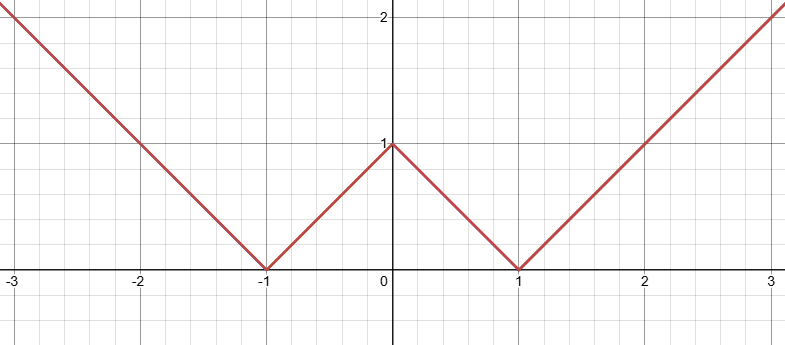
\includegraphics[width=0.6\linewidth]{images/PW.png}
\caption{Кусочно-линейная функция}
\label{fig:PW}
\end{figure}

\begin{figure}
\centering
\vspace*{0.7cm}
\includegraphics[width=0.5\linewidth]{images/"Spline".png}
\caption{Сглаживающий сплайн}
\label{fig:Spline}
\end{figure}

Коэффициенты решения для сглаживающего сплайна выглядит следующим образом: $q = \left[2.5, -0.0117, 2.48, -0.0673, 0.0488, -3.35\right]$.

Тестовые входные данные с координатами точек хранятся в директории \text{/SciDevOOP/bin/Resources}. Содержимое этих файлов представлено в таблице \ref{tab:testData}.

\begin{table}
	\caption{Содержимое файлов с входными данными}
	\centering
	\small
	\begin{tabularx}{1.0\textwidth}{| >{\raggedright\arraybackslash}X | >{\raggedright\arraybackslash}X | >{\raggedright\arraybackslash}X | >{\raggedright\arraybackslash}X |}
		\hline
		\centering{Линейная 3-х мерная}  & \centering{Полином} & \centering{Кусочно-постоянная} & \centering{Сплайн} \tabularnewline \hline    
			\text{7}\newline
			\text{0 0 1} \newline
			\text{1 0 2} \newline
			\text{0 1 2} \newline
			\text{1 1 3} \newline
			\text{0,5 0 1,5} \newline
			\text{0 0,5 1,5} \newline
			\text{0,5 0,5 2} \newline  & 
			\text{15} \newline
			\text{-2,5 27,875} \newline
			\text{-2 15} \newline
			\text{-1,5 6,625} \newline
			\text{-1 2} \newline
			\text{-0,5 0,375} \newline
			\text{0 1} \newline
			\text{0,5 3,125} \newline
			\text{1 6} \newline
			\text{1,5 8,875} \newline
			\text{2 11} \newline
			\text{2,5 11,625} \newline
			\text{3 10} \newline
			\text{3,5 5,375} \newline
			\text{4 -3} \newline
			\text{4,5 -15,87} \newline & 
			\text{9} \newline
			\text{-2 1} \newline
			\text{-1,5 0,5} \newline
			\text{-1 0} \newline
			\text{-0,5 0,5} \newline
			\text{0 1} \newline
			\text{0,5 0,5} \newline
			\text{1 0} \newline
			\text{1,5 0,5} \newline
			\text{2 1} & 
			\text{11} \newline
			\text{0,0 2,5} \newline
			\text{0,5 2,5} \newline
			\text{1,1 2,5} \newline
			\text{1,5 2,5} \newline
			\text{2,0 2,5} \newline
			\text{2,5 2,5} \newline
			\text{3,0 2,5} \newline
			\text{4,0 2,3} \newline
			\text{4,5 1,2} \newline
			\text{4,8 0,8} \newline
			\text{5,0 0,0} \newline \tabularnewline \hline    
	\end{tabularx}
	\label{tab:testData}
\end{table}

\section{Тестирование метода имитации отжига}


\begin{table}
	\caption{Тестирование 3-х мерной линейной функции $P(\vec{x}) = 1 + x_1 + x_2$.}
	\centering
	\small
	\begin{tabularx}{1.0\textwidth}{| >{\centering\arraybackslash}X | >{\raggedright\arraybackslash}X | >{\raggedright\arraybackslash}X |}
		\hline
		\centering{Начальные параметры}  & \centering{Функционал} & \centering{Средний результат из 10 решений} \tabularnewline \hline    
		
		\multirow{4}{*}{\centering{(0.89; 0.5; 0.5)}} & $L_1$ & \centering{9.985284E-001, 1.000726E+000, 1.001621E+000} \tabularnewline \cline{2-3}
	
		 & $L_2$ & \centering{1.003186E+000, 9.977719E-001,	9,964673E-001} \tabularnewline \cline{2-3}
	
		 & $L_{\inf}$ & \centering{9.988302E-001, 1.003419E+000, 9.985865E-001} \tabularnewline \cline{2-3}
	
		 & Интеграл & \centering{0.00000000E+000; 0.00000000E+000; 0.00000000E+000} \tabularnewline \hline
	\end{tabularx}
	\label{tab:testLineN1}
\end{table}

\begin{table}
	\caption{Тестирование кусочно-линейной функции $f(x) = -1 + |x + 1| + |x| + |x - 1|$.}
	\centering
	\small
	\begin{tabularx}{1.0\textwidth}{| >{\raggedright\arraybackslash}X | >{\raggedright\arraybackslash}X | >{\raggedright\arraybackslash}X |}
		\hline
		\centering{Начальные параметры}  & \centering{Функционал} & \centering{Средний результат из 10 решений} \tabularnewline \hline    
		
		\multirow{4}{*}{\raggedleft
			\begin{tabular}{c}
				 0.8, \\
				 0.7, \\
				 0.9, -0.78, -1.87, \\
				 -1.0, 0.0, 1.0
			\end{tabular}
		} & $L_1$ & \centering{2.864295E-002, -1.044582E+000, 9.740291E-001, -9.856934E-001, 1.033343E+000} \tabularnewline \cline{2-3}
		
		& $L_2$ & \centering{9.581629E-004, -1.100468E+000, 1.060370E+000, -1.067029E+000, 1.081162E+000} \tabularnewline \cline{2-3}
		
		& $L_{\inf}$ & \centering{-1,847915E-002, -9.562990E-001, 9.900883E-001, -9.708578E-001, 9.495355E-001} \tabularnewline \cline{2-3}
		
		& Интеграл & \centering{0.00000000E+000; 0.00000000E+000; 0.00000000E+000} \tabularnewline \hline
	\end{tabularx}
	\label{tab:testPW1}
\end{table}

\begin{table}
	\caption{Тестирование полиномиальной функции $P(x) = 1 + 3x + 3x^2 - x^3$.}
	\centering
	\small
	\begin{tabularx}{1.0\textwidth}{| >{\raggedright\arraybackslash}X | >{\raggedright\arraybackslash}X | >{\raggedright\arraybackslash}X |}
		\hline
		\centering{Начальные параметры}  & \centering{Функционал} & \centering{Средний результат из 10 решений} \tabularnewline \hline    
		
		\multirow{4}{*}{\centering{(0.8, 0.7, 0.9, -0.28)}} & $L_1$ & \centering{9.760448E-001, 3.056967E+000, 3.025434E+000,	-1.009347E+000} \tabularnewline \cline{2-3}
		
		& $L_2$ & \centering{1.043514E+000, 2.921941E+000, 3.004910E+000, -9.983161E-001} \tabularnewline \cline{2-3}
		
		& $L_{\inf}$ & \centering{1.127008E+000, 3.080072E+000, 3.011509E+000, -1.007120E+000} \tabularnewline \cline{2-3}
		
		& Интеграл & \centering{0.00000000E+000; 0.00000000E+000; 0.00000000E+000} \tabularnewline \hline
	\end{tabularx}
	\label{tab:testPolynomial1}
\end{table}

\begin{table}
	\caption{Тестирование сплайна.}
	\centering
	\small
	\begin{tabularx}{1.0\textwidth}{| >{\raggedright\arraybackslash}X | >{\raggedright\arraybackslash}X | >{\raggedright\arraybackslash}X |}
		\hline
		\centering{Начальные параметры}  & \centering{Функционал} & \centering{Средний результат из 10 решений} \tabularnewline \hline    
		
			\multirow{4}{*}{\raggedleft
			\begin{tabular}{c}
				0.5, 0.0, 1.47, -0.78, 1.88,\\
				 -0.35, \\
				0.0, 2.0, 5.0
			\end{tabular}
		} & $L_1$ & \centering{2.572843E+000, -3.772355E-001, 2.486581E+000, -2.242274E-001, 2.995627E-002, -3.614091E+000} \tabularnewline \cline{2-3}
		
		& $L_2$ & \centering{2.500145E+000, -1.446680E-001, 2.490407E+000, -9.458615E-002, 2.340403E-002, -3.365737E+000} \tabularnewline \cline{2-3}
		
		& $L_{\inf}$ & \centering{2.399551E+000, 1.817553E-001, 2.490943E+000, -6.092797E-002, 2.510118E-002, -3.336969E+000} \tabularnewline \cline{2-3}
		
		& Интеграл & \centering{0.00000000E+000; 0.00000000E+000; 0.00000000E+000} \tabularnewline \hline
	\end{tabularx}
	\label{tab:testSpline1}
\end{table}

\section{Тестирование метода сопряжённых градиентов}

\begin{table}
	\caption{Тестирование 3-х мерной линейной функции $P(\vec{x}) = 1 + x_1 + x_2$.}
	\centering
	\small
	\begin{tabularx}{1.0\textwidth}{| >{\raggedright\arraybackslash}X | >{\raggedright\arraybackslash}X | >{\raggedright\arraybackslash}X |}
		\hline
		\centering{Начальные параметры}  & \centering{Функционал} & \centering{Результат} \tabularnewline \hline    
		
		\multirow{2}{*}{\centering{(-1.5; 0.1; 1.0)}} & $L_1$ & \centering{1.000000E+000, 1.000000E+000, 1.000000E+000} \tabularnewline \cline{2-3}
		
		& $L_2$ & \centering{1.000000E+000, 9.999999E-001, 9.999998E-001} \tabularnewline \hline
	\end{tabularx}
	\label{tab:testLineN2}
\end{table}

\begin{table}
	\caption{Тестирование кусочно-линейной функции $f(x) = -1 + |x + 1| + |x| + |x - 1|$.}
	\centering
	\small
	\begin{tabularx}{1.0\textwidth}{| >{\raggedright\arraybackslash}X | >{\raggedright\arraybackslash}X | >{\raggedright\arraybackslash}X |}
		\hline
		\centering{Начальные параметры}  & \centering{Функционал} & \centering{Результат} \tabularnewline \hline    
		
		\multirow{4}{*}{\raggedleft
		\begin{tabular}{c}
			0.7, \\
			0.4, \\
			0.1, 0.1, 0.2, \\
			-1.0, 0.0, 1.0 \\
		\end{tabular}} & $L_1$ & \centering{7.003582E-002, -8.814619E-001, 8.784511E-001, -9.392526E-001, 9.824676E-001} \tabularnewline \cline{2-3}
		
		& $L_2$ & \centering{2,217045E-01
			7,360733E-02
			-7,448983E-02
			7,741301E-02
			3,293158E-01} \tabularnewline \hline
	\end{tabularx}
	\label{tab:testPW2}
\end{table}


\section{Тестирование метода Левенберга — Марквардта}

\begin{table}
	\caption{Тестирование 3-х мерной линейной функции $P(\vec{x}) = 1 + x_1 + x_2$.}
	\centering
	\small
	\begin{tabularx}{1.0\textwidth}{| >{\raggedright\arraybackslash}X | >{\raggedright\arraybackslash}X | >{\raggedright\arraybackslash}X |}
		\hline
		\centering{Начальные параметры}  & \centering{Функционал} & \centering{Результат} \tabularnewline \hline    
		
		\multirow{4}{*}{\centering{(-1.0, 0.1, 2.0)}} & $L_2$ & \centering{1.000000E+000, 1.000000E+000, 1.000000E+000} \tabularnewline \hline
	\end{tabularx}
	\label{tab:testLineN3}
\end{table}

\begin{table}
	\caption{Тестирование кусочно-линейной функции $f(x) = -1 + |x + 1| + |x| + |x - 1|$.}
	\centering
	\small
	\begin{tabularx}{1.0\textwidth}{| >{\raggedright\arraybackslash}X | >{\raggedright\arraybackslash}X | >{\raggedright\arraybackslash}X |}
		\hline
		\centering{Начальные параметры}  & \centering{Функционал} & \centering{Результат} \tabularnewline \hline    
		
		\multirow{4}{*}{\raggedleft
			\begin{tabular}{c}
				0.7, \\
				0.4, \\
				0.1, 0.1, 0.2, \\
				-1.0, 0.0, 1.0 \\
		\end{tabular}} & $L_2$ & \centering{9.585372E-15, -1.000000E+00, 1.000000E+00, -1.000000E+00, 1.000000E+00} \tabularnewline \hline
		
	\end{tabularx}
	\label{tab:testPW3}
\end{table}
%\chapter*{Заключение}

\addcontentsline{toc}{chapter}{Заключение}


Мир, в котором мы живем, состоит из разнообразных регионов, каждый из которых имеет уникальный набор проблем и проблем. Эти региональные проблемы могут варьироваться от экологических проблем, таких как загрязнение и изменение климата, до социальных и экономических проблем, таких как бедность и безработица. Решение этих проблем имеет решающее значение для устойчивого развития и благополучия затронутых регионов и их жителей.

\newpage
%
\chapter*{Приложение. Текст программы.}
\addcontentsline{toc}{chapter}{Приложение. Текст программы}
\label{code: code}
\subsection*{FEM2D.h}
\lst{cpp}{code/FEM2D.h}

\subsection*{FEM2D.cpp}
\lst{cpp}{code/FEM2D.cpp}

\subsection*{FEM3D.h}
\lst{cpp}{code/FEM3D.h}

\subsection*{FEM3D.cpp}
\lst{cpp}{code/FEM3D.cpp}

\subsection*{ITimeScheme.h}
\lst{cpp}{code/ITimeScheme.h}

\subsection*{ImplicitScheme.h}
\lst{cpp}{code/ImplicitScheme.h}

\subsection*{ImplicitScheme.cpp}
\lst{cpp}{code/ImplicitScheme.cpp}

\subsection*{PardisoSolver.h}
\lst{cpp}{code/PardisoSolver.h}

\subsection*{PardisoSolver.cpp}
\lst{cpp}{code/PardisoSolver.cpp}

\subsection*{DirectTask.h}
\lst{cpp}{code/DirectTask.h}

\subsection*{DirectTask.cpp}
\lst{cpp}{code/DirectTask.cpp}

\subsection*{GeometryInverseTask.h}
\lst{cpp}{code/GeometryInverseTask.h}

\subsection*{GeometryInverseTask.cpp}
\lst{cpp}{code/GeometryInverseTask.cpp}

\subsection*{Source.cpp}
\lst{cpp}{code/Source.cpp}

\end{document}